\documentclass[12pt]{article}
\usepackage[utf8]{inputenc}
\usepackage[T1]{fontenc}
\usepackage{graphicx}
\usepackage[a4paper, margin=1in]{geometry}
\usepackage{hyperref}
\usepackage{listings}
\usepackage{xcolor}
\usepackage{caption}
\usepackage{tikz}
\usetikzlibrary{shapes.geometric, arrows.meta, positioning, shadows}

\hypersetup{
    colorlinks=true,
    linkcolor=blue,
    filecolor=magenta,      
    urlcolor=cyan,
    pdftitle={IntelliDiff Project Report},
    pdfpagemode=FullScreen,
}

\definecolor{codegreen}{rgb}{0,0.6,0}
\definecolor{codegray}{rgb}{0.5,0.5,0.5}
\definecolor{codepurple}{rgb}{0.58,0,0.82}
\definecolor{backcolour}{rgb}{0.98,0.98,0.98}
\definecolor{keywordblue}{rgb}{0.1, 0.2, 0.7}

\lstdefinelanguage{TypeScript}{
  keywords={
    break, case, catch, continue, debugger, default, delete, do, else,
    finally, for, function, if, in, instanceof, new, return, switch,
    this, throw, try, typeof, var, void, while, with,
    % TypeScript-specific keywords
    as, any, async, await, boolean, constructor, declare, get, implements,
    interface, let, module, number, private, protected, public, set,
    string, super, type, enum, export, extends, import, from, is, null,
    undefined, require
  },
  morecomment=[l]{//},
  morecomment=[s]{/*}{*/},
  morestring=[b]{`},
  morestring=[b]{'},
  morestring=[b]{"},
  sensitive=true
}

\lstdefinestyle{mystyle}{
    backgroundcolor=\color{backcolour},   
    commentstyle=\itshape\color{codegreen},
    keywordstyle=\bfseries\color{keywordblue},
    numberstyle=\tiny\color{codegray},
    stringstyle=\color{codepurple},
    basicstyle=\ttfamily\footnotesize,
    breakatwhitespace=false,         
    breaklines=true,                 
    captionpos=b,                    
    keepspaces=true,                 
    numbers=left,                    
    numbersep=5pt,                  
    showspaces=false,                
    showstringspaces=false,
    showtabs=false,                  
    tabsize=2,
    frame=single,
    framerule=0.5pt
}

\lstset{style=mystyle}

\title{IntelliDiff: AI-Powered Git History Analysis}
\author{Team 01}
\date{\today}

\begin{document}

\maketitle

\begin{abstract}
    This report details the design and implementation of ``IntelliDiff,'' a Cursor extension that supercharges the popular Git Graph plugin with Artificial Intelligence. The primary goal of this project is to simplify the understanding of complex Git histories by providing intelligent, automated analysis of code changes. Key features include AI-powered summaries for commits, comparisons between different versions, and in-depth analysis of a single file's evolution over time. To ensure a fluid user experience and mitigate the inherent latency of AI models, the extension implements a sophisticated architecture featuring asynchronous processing for non-blocking UI updates and a two-tier caching system (memory and disk) to dramatically reduce response times and API costs on repeated analyses. This project demonstrates a practical application of Large Language Models (LLMs) to enhance developer productivity and streamline code review processes.
\end{abstract} 

\section{Motivation and Significance}
In modern software development, projects often involve hundreds of contributors and tens of thousands of commits, resulting in highly complex and non-linear Git histories. Understanding this history is crucial for many development tasks, including code reviews, bug tracking, and onboarding new team members. However, manually inspecting `git log` outputs or raw diffs is a time-consuming and cognitively demanding process. Developers often struggle to grasp the high-level purpose of a set of changes, focusing on line-by-line details rather than the overall architectural or business logic impact.

This challenge is exacerbated in large, long-lived repositories where the context behind historical changes can be lost over time. A developer trying to understand a legacy module might spend hours, or even days, piecing together its evolution through a tangled web of commits. Similarly, code reviewers are under pressure to provide quick yet thorough feedback, a task made difficult by large pull requests with dozens of file changes.

This project, ``IntelliDiff,'' is motivated by the opportunity to address these inefficiencies through the power of Large Language Models (LLMs). By integrating AI-driven analysis directly into the Git visualization workflow, we can automate the cognitive task of summarizing and interpreting code changes. Instead of asking developers to manually decipher diffs, we can provide them with concise, high-level summaries that explain the ``what'' and ``why'' of a change, not just the ``how.''

The significance of this project lies in its potential to significantly enhance developer productivity and improve the quality of code collaboration. By reducing the time and effort required to understand code evolution, we can:
\begin{itemize}
    \item \textbf{Accelerate Code Reviews:} Reviewers can quickly understand the purpose and impact of changes, allowing them to focus on providing higher-level feedback.
    \item \textbf{Simplify Onboarding:} New developers can get up to speed on a codebase faster by reviewing AI-generated summaries of key modules' histories.
    \item \textbf{Improve Code Archaeology:} Investigating legacy code or tracking down the origin of a bug becomes more efficient when historical changes are automatically summarized.
    \item \textbf{Democratize Understanding:} It lowers the barrier for all stakeholders, including less technical ones, to understand the progress and evolution of a software project.
\end{itemize}

In essence, this project aims to shift the burden of understanding complex code history from the human developer to the AI, freeing up valuable cognitive resources for more creative and critical problem-solving tasks. 

\section{Software Description}
The extension is built upon a robust, decoupled three-tier architecture that separates concerns between the user interface, the core business logic, and the AI processing. This design ensures modularity, scalability, and maintainability.

\subsection{Software Architecture}
The system is composed of three primary components that work in concert: the Webview Frontend, the Cursor Extension Backend, and a Python-based AI Service. The interaction between these components is illustrated in Figure \ref{fig:architecture}.

\begin{figure}[h!]
    \centering
    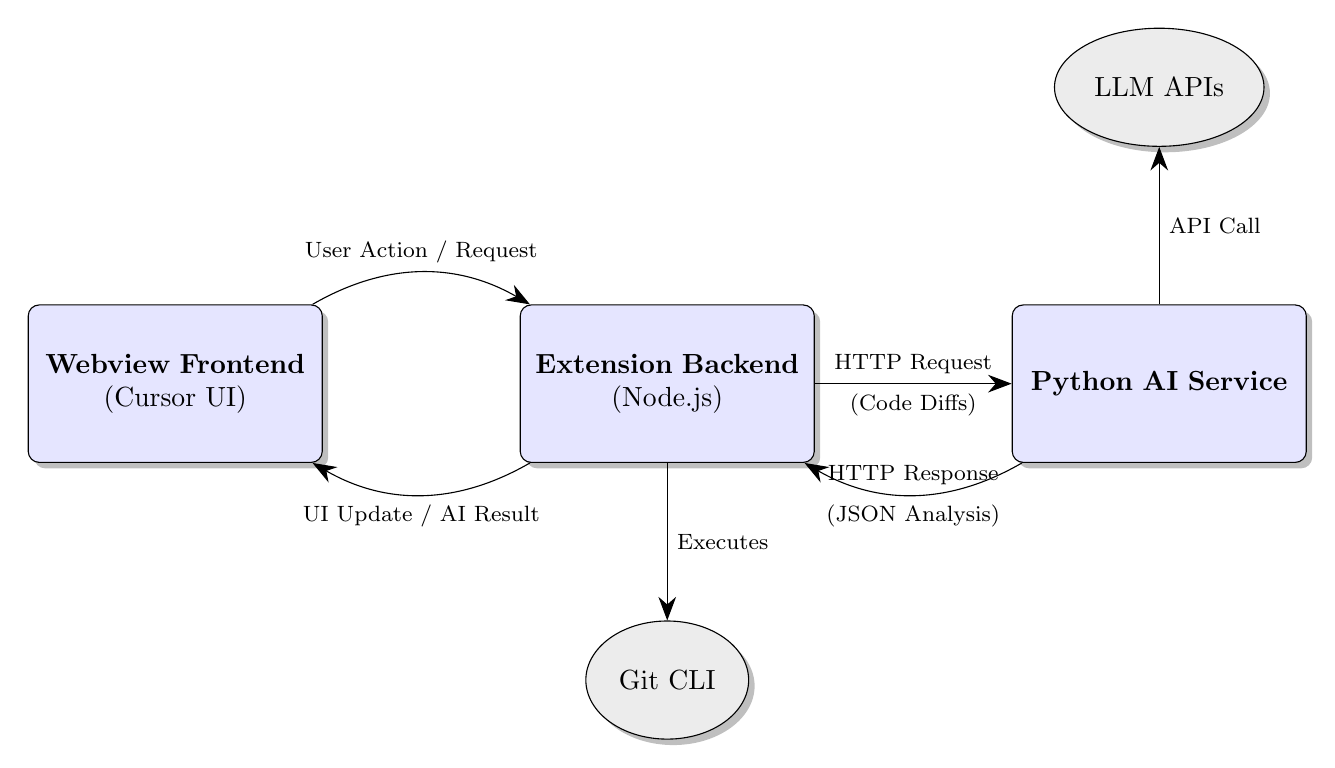
\begin{tikzpicture}[
        node distance=2cm and 2.5cm,
        block/.style={
            rectangle, 
            draw, 
            text width=3.5cm, 
            minimum height=2cm, 
            text centered, 
            rounded corners, 
            fill=blue!10,
            drop shadow
        },
        cloud/.style={
            ellipse,
            draw,
            minimum height=1.5cm,
            fill=gray!15,
            drop shadow
        },
        line/.style={
            draw, 
            -{Stealth[length=3mm]},
            font=\footnotesize
        }
    ]
    % Nodes
    \node[block] (frontend) {\textbf{Webview Frontend} \\ (Cursor UI)};
    \node[block, right=of frontend] (backend) {\textbf{Extension Backend} \\ (Node.js)};
    \node[block, right=of backend] (aiservice) {\textbf{Python AI Service}};
    \node[cloud, above=of aiservice] (llm_apis) {LLM APIs};
    \node[cloud, below=of backend] (git) {Git CLI};

    % Arrows
    \path[line] (frontend) edge[bend left] node[above] {User Action / Request} (backend);
    \path[line] (backend) edge[bend left] node[below] {UI Update / AI Result} (frontend);
    \path[line] (backend) edge node[above] {HTTP Request} node[below] {(Code Diffs)} (aiservice);
    \path[line] (aiservice) edge[bend left] node[above] {HTTP Response} node[below] {(JSON Analysis)} (backend);
    \path[line] (backend) edge node[right, midway] {Executes} (git);
    \path[line] (aiservice) edge node[right, midway] {API Call} (llm_apis);
    \end{tikzpicture}
    \caption{The three-tier architecture of the IntelliDiff extension, showing the flow of requests and data between the Webview UI, the Cursor Extension Backend, and the Python AI Service.}
    \label{fig:architecture}
\end{figure}

\begin{enumerate}
    \item \textbf{Webview Frontend}: This is the user-facing component, rendered inside a Cursor Webview panel. It is responsible for all visualization, including the Git graph itself, commit details, and the display of AI-generated analysis. It is built with standard web technologies (TypeScript, HTML, CSS) and communicates with the backend via a message-passing API provided by Cursor. When a user interacts with the graph (e.g., clicks on a commit), the frontend sends a request message to the backend.

    \item \textbf{Cursor Extension Backend}: Running in a Node.js environment, this is the core of the extension. It acts as the central orchestrator, handling requests from the frontend, managing application state, and interfacing with external services. Its key responsibilities include:
    \begin{itemize}
        \item Executing native Git commands to fetch repository data (logs, diffs, etc.).
        \item Implementing the business logic for performance optimizations, such as asynchronous processing and caching.
        \item Communicating with the Python AI Service via HTTP requests, sending it data to be analyzed.
        \item Pushing data and updates (including asynchronous AI results) back to the frontend.
    \end{itemize}

    \item \textbf{Python AI Service}: This is a lightweight, local web server dedicated to handling all interactions with Large Language Models (supporting both OpenAI and DeepSeek APIs). Decoupling the AI logic into a separate service provides several advantages: it allows for the use of Python's mature data science and AI ecosystem, it isolates API keys and prompts from the main extension code, and it could potentially be deployed remotely in the future. It receives diff content and other metadata from the extension backend, constructs detailed prompts, and returns structured analysis results.
\end{enumerate}

\subsection{Core AI Features and Optimizations}
The project's main innovation lies in its deep integration of AI analysis and the performance optimizations that make it practical for daily use.

\subsubsection{Multi-faceted AI Analysis}
Based on the context, the extension can perform several types of AI analysis by sending structured prompts to the AI service. The prompts are carefully engineered to elicit concise and relevant information:
\begin{itemize}
    \item \textbf{Comprehensive Commit Analysis}: For a single commit, the AI is asked to generate a holistic summary covering the main purpose, affected modules, technical and business value, and overall code quality.
    \item \textbf{Version Comparison Analysis}: When comparing two commits, the AI focuses on summarizing the evolutionary changes, such as new features, refactoring efforts, and architectural shifts.
    \item \textbf{Dedicated File History View}: In a particularly powerful feature, the extension can open a detailed history for a single file in a new, dedicated tab. This view offers two modes of AI analysis:
    \begin{itemize}
        \item \textit{Evolution Analysis}: The AI analyzes the file's entire commit history to produce a report on its development patterns, identify key historical changes, and provide optimization recommendations.
        \item \textit{Targeted Version Comparison}: Within the history view, users can select any two versions of the file and receive a specific, AI-powered comparison of just those two points in time.
    \end{itemize}
\end{itemize}

\subsubsection{Optimization 1: Asynchronous Processing}
To avoid blocking the UI while waiting for (potentially slow) AI responses, the extension employs an asynchronous, non-blocking workflow.
\begin{enumerate}
    \item A user action triggers a request to the backend.
    \item The backend \textit{immediately} returns the basic, non-AI-dependent data (e.g., commit metadata, file list). The frontend renders this information instantly, showing a loading indicator for the AI section.
    \item In parallel, the backend spawns an asynchronous task to prepare data and call the AI service.
    \item Once the AI analysis is complete, the backend pushes the result to the frontend using a dedicated message, which then dynamically updates the UI.
\end{enumerate}
This ``instant-feedback, progressive-enhancement'' model is critical for maintaining a responsive user experience.

\subsubsection{Optimization 2: Two-Tier Intelligent Caching}
To minimize API costs and accelerate repeated analyses, the extension uses a sophisticated two-tier caching system.
\begin{itemize}
    \item \textbf{L1 Memory Cache}: A simple `Map` object for ultra-fast (sub-millisecond) access to results within the current session. It is managed by a Least Recently Used (LRU) eviction policy.
    \item \textbf{L2 Disk Cache}: A JSON file on disk that persists results across sessions. When the extension starts, it pre-loads a portion of the disk cache into memory for faster initial access.
    \item \textbf{Intelligent Cache Key}: The cache key is not the commit hash. Instead, it is a `sha256` hash of the code diff content itself. This is a crucial optimization: if the same change is present in two different commits (e.g., from a cherry-pick or rebase), the system recognizes it and reuses the cached result, saving a redundant API call.
\end{itemize}

\subsection{Implementation Highlights}
Below are two code snippets from the TypeScript backend that illustrate the implementation of the core optimization strategies.

\subsubsection{Asynchronous AI Analysis Workflow}
The following snippet from `dataSource.ts` shows how a request for commit details is handled. It immediately returns the basic details while launching the AI analysis in the background.

\begin{lstlisting}[language=TypeScript, caption={Simplified from src/dataSource.ts}, label={lst:async}]
// Simplified from src/dataSource.ts
public async getCommitDetails(repo: string, commitHash: string) {
    // 1. Fetch basic details using Git commands
    const commitDetails = await this.getCommitDetailsBase(repo, commitHash);
    
    // 2. Immediately return the basic details for instant UI rendering
    const result = { commitDetails: commitDetails, error: null };

    // 3. Trigger the asynchronous AI analysis in the background.
    // This does not block the return of the function.
    if (aiConfig.enabled) {
        this.performAsyncCommitAnalysis(
            repo, commitHash, commitDetails, ...
        ).catch(error => {
            this.logger.logError(`Async AI analysis failed: ${error}`);
        });
    }

    return result;
}

// Later, inside performAsyncCommitAnalysis...
const aiAnalysis = await this.generateComprehensiveCommitAnalysis(...);
// Push the result to the UI via a registered callback
this.sendAIAnalysisUpdate(commitHash, null, aiAnalysis);
\end{lstlisting}

\subsubsection{Intelligent Cache Key Generation}
This snippet from `aiCache.ts` demonstrates the smart cache key generation, which is fundamental to the efficiency of the caching system.

\begin{lstlisting}[language=TypeScript, caption={From src/aiCache.ts}, label={lst:cachekey}]
// From src/aiCache.ts
public generateCacheKey(content: string, type: string = 'default'): string {
    const hash = crypto.createHash('sha256');
    // The key is based on the analysis type and the actual content (diff)
    hash.update(`${type}:${content}`);
    return hash.digest('hex');
}
\end{lstlisting}

\subsubsection{Advanced Git Command Optimization}
A significant performance enhancement was achieved in the File History feature by optimizing Git command execution. The initial approach required multiple (`1 + 3N`) calls to Git for `N` commits. This was consolidated into a single, highly-efficient command that fetches all necessary data in one pass, dramatically reducing process overhead and improving load times from seconds to milliseconds.

\begin{lstlisting}[language=bash, caption={Optimized single-pass Git command for file history}, label={lst:git-optim}]
# Fetches log, author, date, message, and file stats in one command
git log --follow --format=%H|%P|%an|%at|%s --numstat --max-count=50 -- filePath
\end{lstlisting} 

\section{Illustrative Examples}
This section demonstrates the practical application of the extension through two common developer workflows: analyzing a single commit and comparing two different commits.

\subsection{Use Case 1: Analyzing a Single Commit}
A common task for a developer is to understand the changes introduced in a specific commit. This might be during a code review or when debugging a feature.

\begin{enumerate}
    \item \textbf{Action}: The user opens the Git Graph view and clicks on a commit in the graph.
    \item \textbf{Immediate Response}: The Commit Details view opens instantly, showing the commit author, message, and a list of changed files. A loading animation is displayed in the "AI Analysis" section (as shown in Figure \ref{fig:use-case-1-loading}).
    \item \textbf{Asynchronous Update}: After a few seconds, the AI analysis result is pushed to the UI, replacing the loading indicator with a concise, structured summary of the commit's purpose, impact, and quality (see Figure \ref{fig:use-case-1-loaded}).
\end{enumerate}

\begin{figure}[h!]
    \centering
    % TODO: Add a screenshot of the commit details view right after clicking,
    % showing the AI analysis section with a loading spinner/message.
    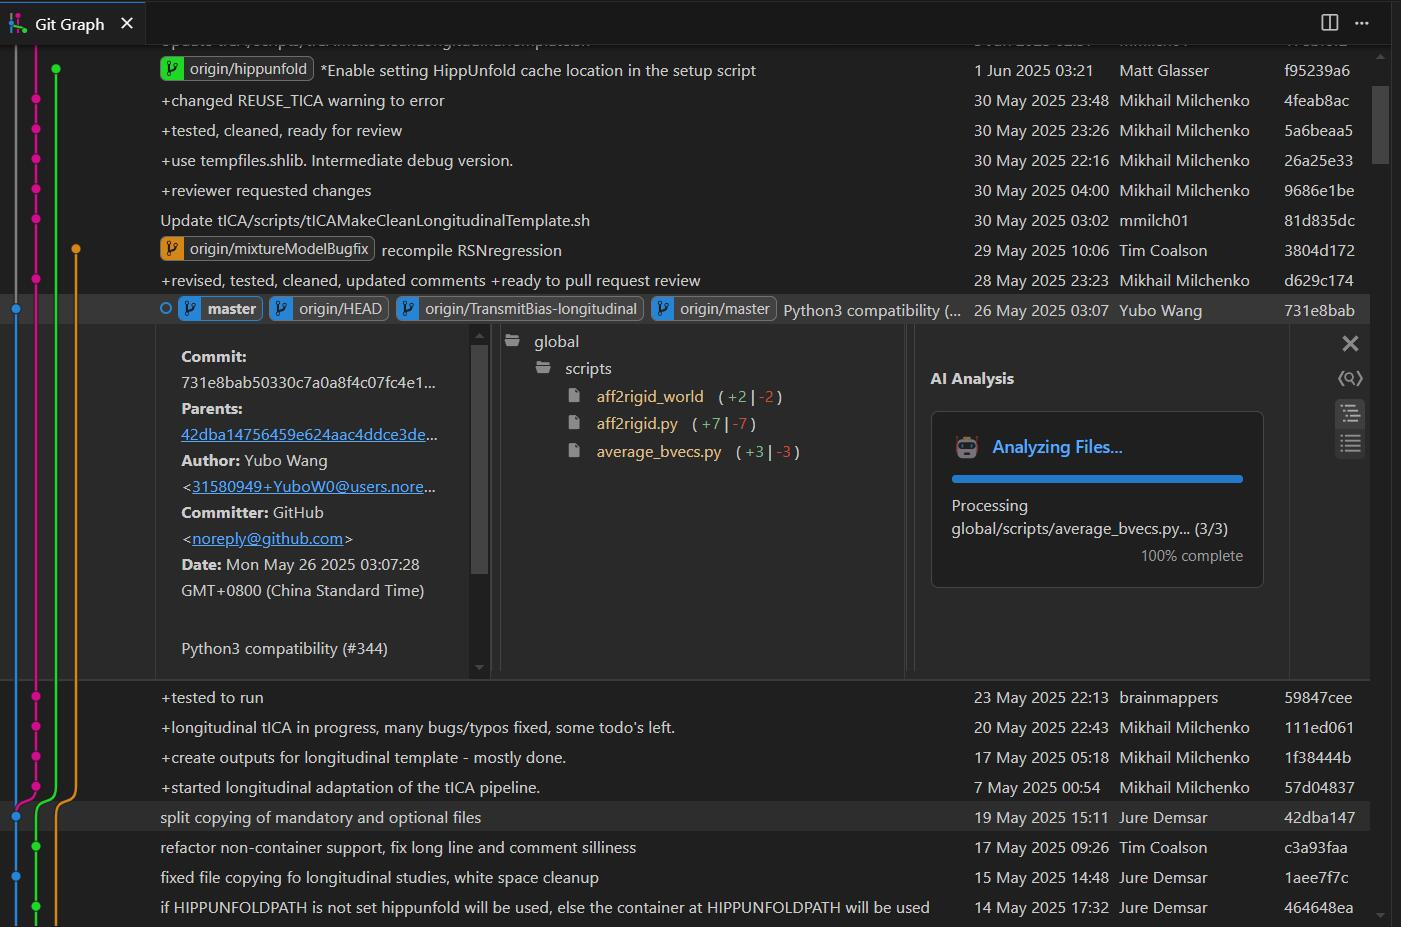
\includegraphics[width=0.9\textwidth]{figures/use-case-1-loading.jpg}
    \caption{The Commit Details view immediately after selection, with the AI Analysis section in a loading state.}
    \label{fig:use-case-1-loading}
\end{figure}

\begin{figure}[h!]
    \centering
    % TODO: Add a screenshot of the same view after the AI analysis has loaded,
    % showing the generated summary.
    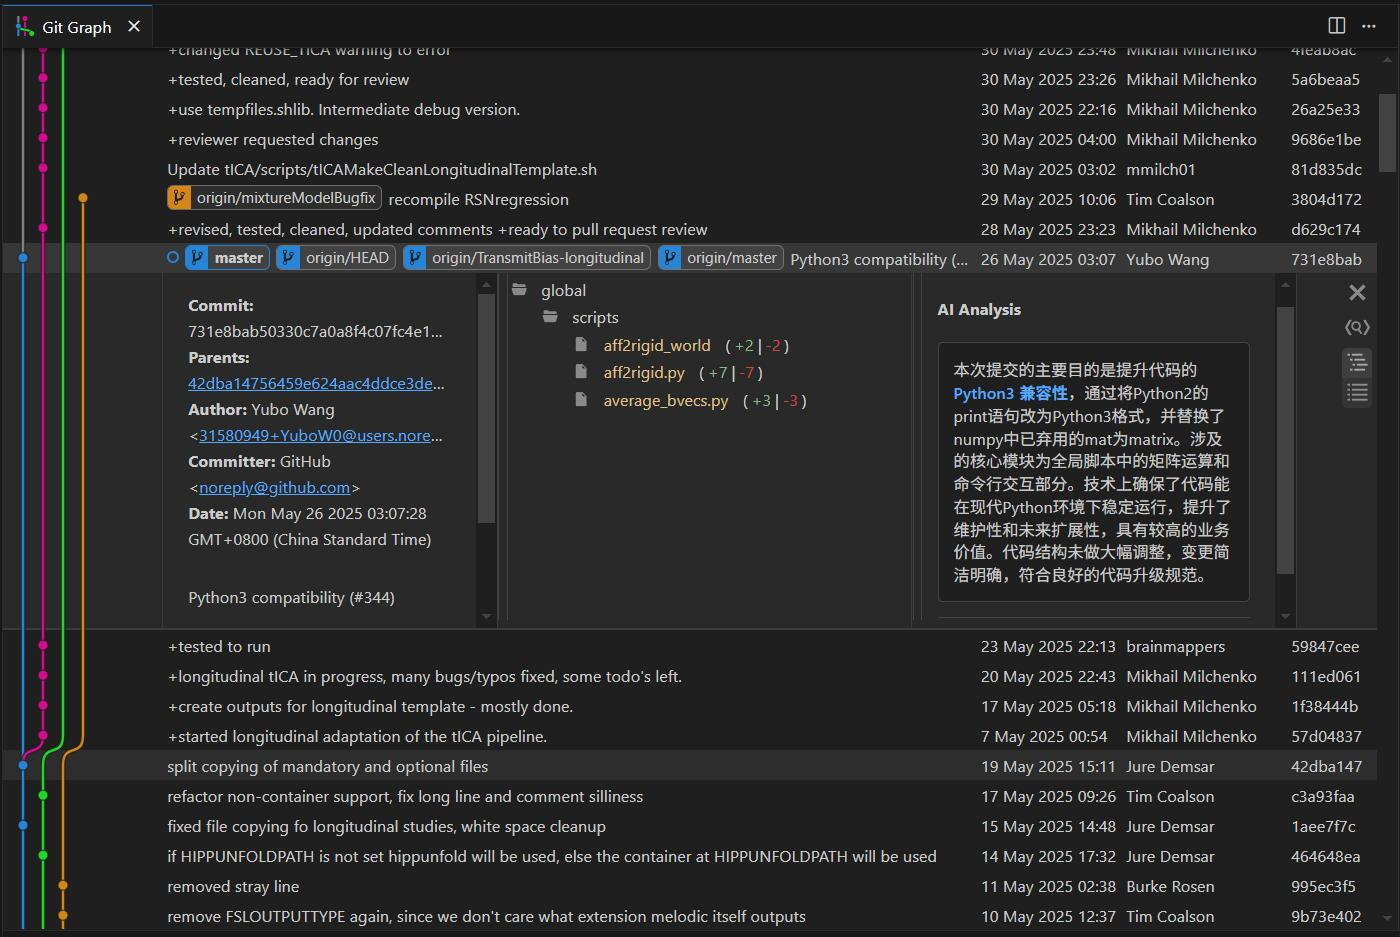
\includegraphics[width=0.9\textwidth]{figures/use-case-1-loaded.jpg}
    \caption{The AI-generated summary is asynchronously loaded and displayed, providing a high-level overview of the changes.}
    \label{fig:use-case-1-loaded}
\end{figure}


\subsection{Use Case 2: Comparing Two Commits}
Another powerful feature is the ability to understand the cumulative changes between any two points in the repository's history, such as comparing a feature branch head against the main branch.

\begin{enumerate}
    \item \textbf{Action}: The user clicks on a commit, then holds CTRL/CMD and clicks on a second commit.
    \item \textbf{Response}: The view immediately lists all files that were changed between these two commits. The AI analysis section shows a loading state.
    \item \textbf{Result}: The AI-generated summary appears, focusing on the high-level evolution between the two versions, highlighting major feature changes or refactoring efforts (as depicted in Figure \ref{fig:use-case-2-comparison}).
\end{enumerate}

\begin{figure}[h!]
    \centering
    % TODO: Add a screenshot of the comparison view, showing the list of changed
    % files and the AI-generated summary of the changes between the two commits.
    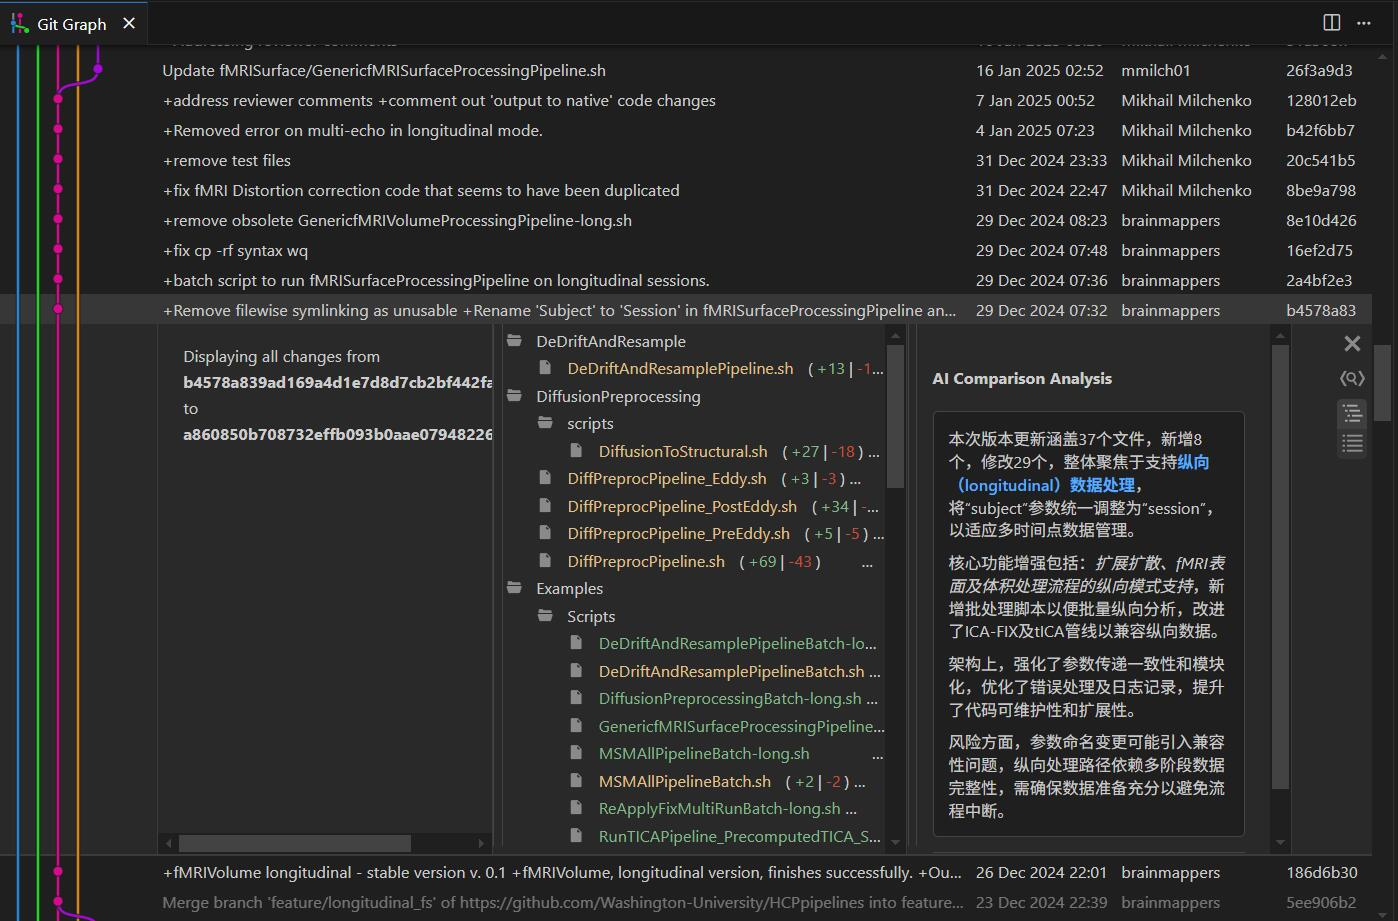
\includegraphics[width=0.9\textwidth]{figures/use-case-2-comparison.jpg}
    \caption{AI analysis of the differences between two commits, summarizing the overall changes.}
    \label{fig:use-case-2-comparison}
\end{figure}

\subsection{Use Case 3: In-Depth File Evolution Analysis}
To understand the full lifecycle of a specific file, developers can use the dedicated File History view.

\begin{enumerate}
    \item \textbf{Action}: In the main Git Graph view, the user right-clicks on a file within the commit details and selects "View File History in New Tab".
    \item \textbf{Evolution Analysis}: A new VS Code tab opens instantly, displaying the file's commit history list and statistics. After a few seconds, the panel is populated with an AI-generated analysis of the file's entire evolution, including key changes and patterns (Figure \ref{fig:use-case-3-history-loaded}).
    \item \textbf{Version Comparison}: The user can then switch to the "Version Compare" tab, select any two commits from the list, and receive a targeted AI analysis comparing just those two versions (Figure \ref{fig:use-case-3-version-compare}).
\end{enumerate}


\begin{figure}[h!]
    \centering
    % TODO: Add a screenshot of the File History tab after the AI analysis is loaded.
    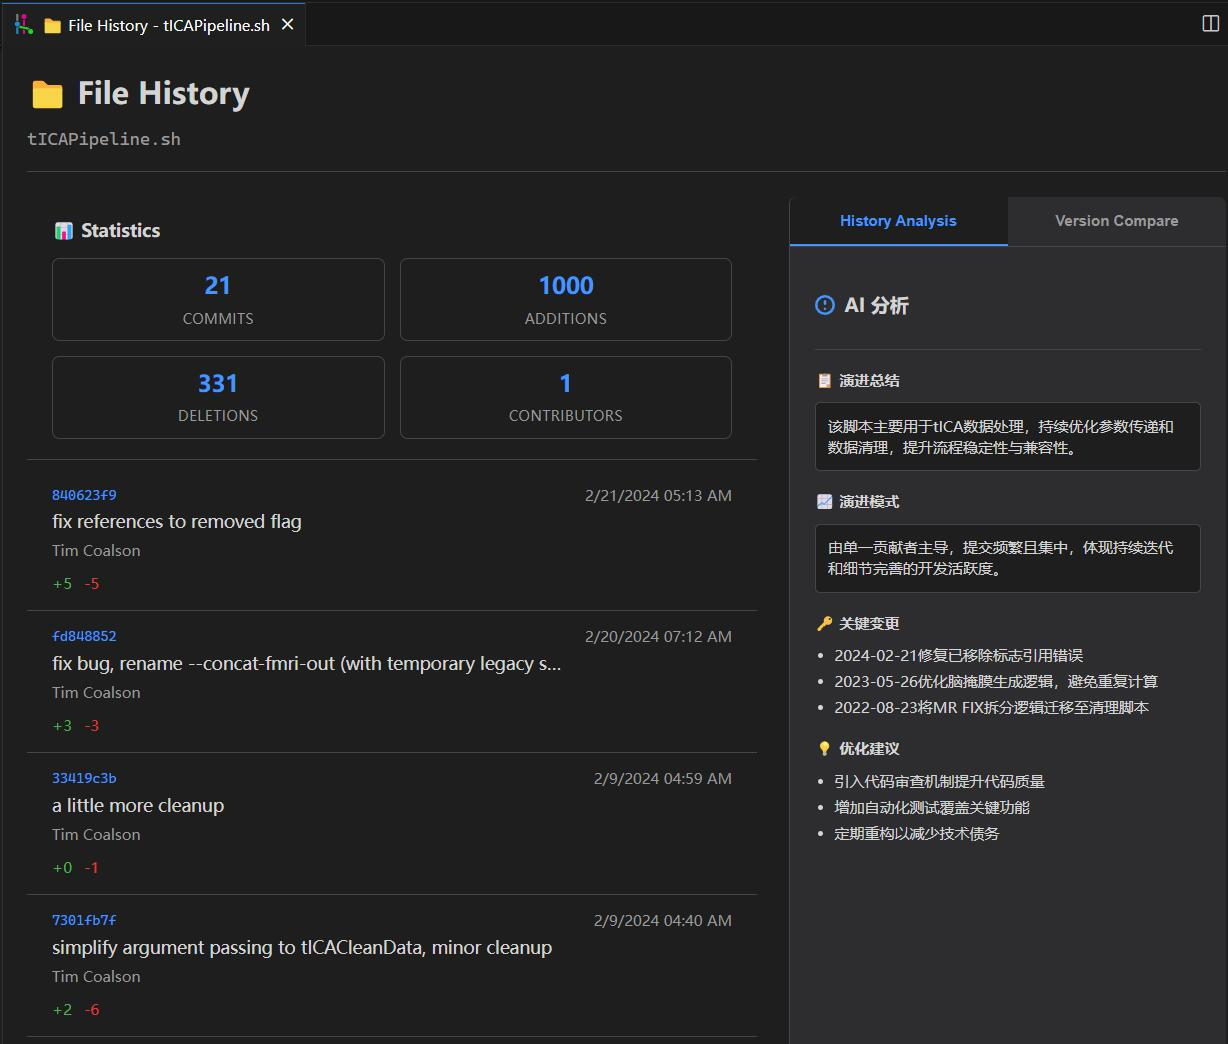
\includegraphics[width=0.9\textwidth]{figures/use-case-3-history-loaded.jpg}
    \caption{The AI analysis, showing the file's evolution summary and patterns.}
    \label{fig:use-case-3-history-loaded}
\end{figure}

\begin{figure}[h!]
    \centering
    % TODO: Add a screenshot of the "Version Compare" tab with two versions selected and compared.
    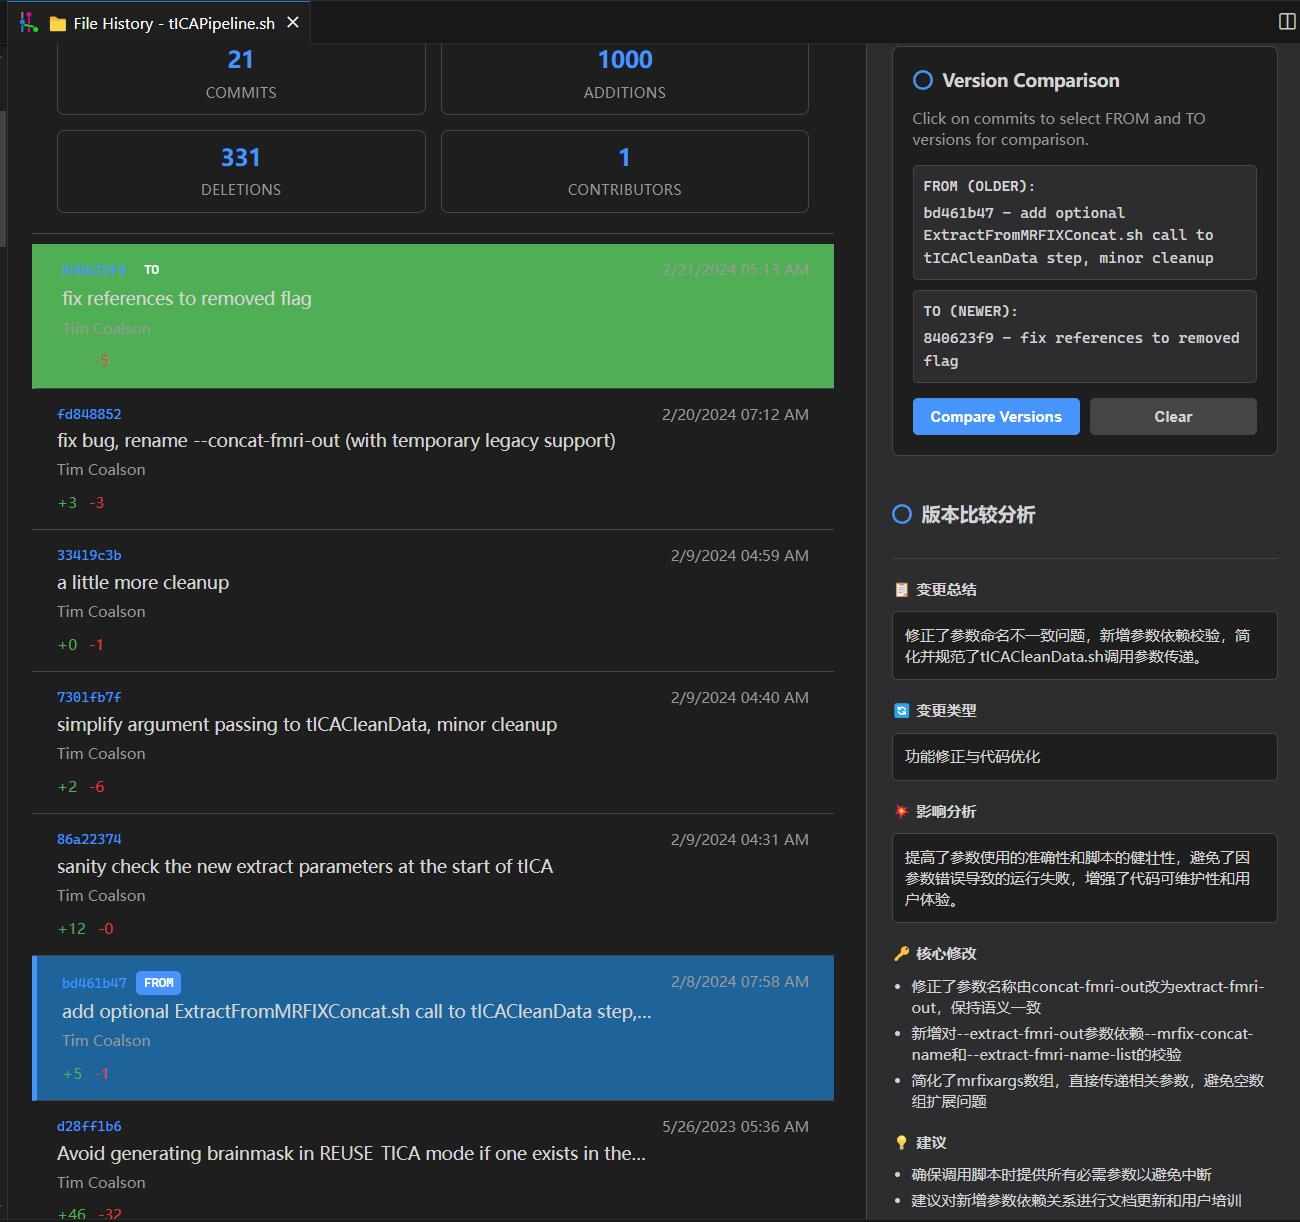
\includegraphics[width=0.9\textwidth]{figures/use-case-3-version-compare.jpg}
    \caption{The "Version Compare" mode, showing a targeted AI analysis between two selected commits for the file.}
    \label{fig:use-case-3-version-compare}
\end{figure} 

\section{Impact}
The introduction of AI-powered analysis into a popular Git visualization tool like Git Graph has a significant and multi-faceted impact on the software development lifecycle. By automating the interpretation of code changes, this project directly addresses key pain points in modern development workflows, leading to measurable improvements in efficiency, quality, and collaboration.

The primary impact is a \textbf{dramatic reduction in cognitive load} for developers. Instead of mentally parsing complex diffs, developers are presented with clear, high-level summaries. This frees up mental energy that can be better spent on architectural considerations, logic validation, and creative problem-solving. This reduction in cognitive overhead leads to several second-order benefits:

\begin{itemize}
    \item \textbf{Increased Development Velocity:} Tasks that require historical context, such as debugging or refactoring, are completed faster. Code reviews can be performed more quickly and efficiently, reducing the time pull requests spend waiting for approval and accelerating the entire development cycle.
    
    \item \textbf{Improved Code Quality and Review Consistency:} By providing an objective, AI-generated summary as a baseline, the tool helps standardize the focus of code reviews. Reviewers are less likely to get lost in minor details and more likely to focus on the significant aspects of a change. This can lead to more consistent and higher-quality feedback, ultimately improving the health of the codebase.
    
    \item \textbf{Enhanced Team Collaboration and Knowledge Sharing:} The tool acts as a knowledge-sharing multiplier. Complex changes become more accessible to all team members, regardless of their initial familiarity with that part of the code. It facilitates better communication during reviews and makes the project history a more valuable and searchable asset. For remote and asynchronous teams, this is particularly impactful, as it provides rich context that might otherwise be lost.
    
    \item \textbf{Faster Onboarding and Learning:} For new members joining a team, the tool is an invaluable learning resource. They can independently explore the history of the codebase and understand the rationale behind key architectural decisions without having to constantly interrupt senior developers. This accelerates their journey to becoming productive contributors.
\end{itemize}

In conclusion, the impact of this project extends beyond a simple productivity boost. It represents a shift towards a more intelligent and context-aware development environment, where developers are augmented by AI to make better-informed decisions faster. It transforms the Git repository from a passive record of changes into an active, intelligent knowledge base. 

\section{Conclusions}
This project successfully demonstrates the feasibility and value of integrating Large Language Models into developer tools to create a more intelligent and efficient Git workflow. By building upon the solid foundation of the Git Graph extension, we have introduced a suite of AI-powered analysis features that address fundamental challenges in understanding and navigating complex code histories, including holistic commit analysis and a dedicated, multi-faceted file history viewer.

The key achievement of this work is the design and implementation of a robust system that is not only powerful in its analytical capabilities but also practical for everyday use. We have shown that by employing a decoupled three-tier architecture, asynchronous processing, and an intelligent two-tier caching system, the inherent latency and cost issues of LLM APIs can be effectively mitigated. The result is a tool that delivers valuable insights without compromising the responsive user experience that developers expect. The intelligent cache key, based on content hashing rather than commit identifiers, is a particularly notable innovation that maximizes cache hits and minimizes redundant processing.

Looking ahead, there are several exciting avenues for future work that could build upon this project's foundation:

\begin{itemize}
    \item \textbf{Deeper Semantic Analysis:} Future versions could be trained to understand the specific domain and conventions of a repository, providing even more context-aware analysis. This could involve fine-tuning models on a per-project basis or using retrieval-augmented generation (RAG) with project documentation.
    
    \item \textbf{Actionable Suggestions:} The AI could move beyond analysis to providing actionable suggestions, such as automatically generating commit messages from uncommitted changes, suggesting potential reviewers for a pull request based on file histories, or identifying related historical commits that might be relevant to a current task.
    
    \item \textbf{Expanded Model Support:} The system already supports multiple API providers (OpenAI, DeepSeek) and could be further expanded to include more models, such as open-source models running locally, to give users more options to balance cost, performance, and privacy.
    
    \item \textbf{Enhanced Team Collaboration Features:} The AI analysis could be integrated into team workflows, such as automatically posting summaries to pull request comments on platforms like GitHub or GitLab, creating a shared understanding of changes for the entire team.
\end{itemize}

In conclusion, ``IntelliDiff'' serves as a compelling proof-of-concept for the future of AI-augmented software development. It illustrates how thoughtful engineering and a focus on user experience can harness the power of AI to transform a fundamental developer tool, making the process of software development faster, smarter, and more collaborative. 

\section*{Acknowledgements}
We would like to express our sincere gratitude to the creator and contributors of the original Git Graph extension. This project would not have been possible without their excellent work in creating a powerful, extensible, and widely-used tool for Git visualization. Their efforts provided the robust foundation upon which our AI enhancements were built. 

\end{document}
